% arara: lualatex: { interaction: nonstopmode, synctex: yes }

\documentclass[../logic-text.tex]{subfiles}
\begin{document}

\chapter{Categorical Logic}
\label{chap:categorical}




Now we turn to some structured logic systems. The first, categorical logic, is one of the oldest. It dates back at least to Aristotle (384--322 BCE). Categorical logic is a fairly simple logic of categories or classes. A class is a group of things that we designate with a common noun: students, teachers, dogs, politicians, etc. Each sentence will use two different classes. One is the subject class, and the other is the predicate class. In this logic, we can say something about all members of a class, called a universal sentence, or we can say something about some members of a class, called a particular sentence. We can also make a positive claim, called an affirmation, or we can make a negative claim, called a negation.

With these two distinctions, universal/particular and affirnation/negation, we can make four kinds of sentences. S and P stand for the subject class and the predicate class, respectively.

\begin{description}
\item[A]: All S are P (universal affirmation)
\item[E]: No S are P (universal negation)
\item[I]: Some S are P (particular affirmation)
\item[O]: Some S are not P (particular negation)\footnote{The letters A, E, I, and O, are thought to come from the first two vowels of the Latin words \emph{affirmo} and \emph{nego}, meaning \enquote{I affirm} and \enquote{I deny.}
} 
\end{description}

Here are some examples of categorical statements, some true and some false.

\begin{enumerate}
\item All dogs are mammals.
\item All mammals are dogs.
\item No reptiles are dogs.
\item No politicians are honest people.
\item Some politicians are honest people.
\item Some cats are amphibians.
\item Some dogs are not beagles.
\item Some beagles are not dogs.
\end{enumerate}

Look at the sentences carefully. You should be able to tell that the odd-numbered ones are true and the even-numbered ones are false.

\section{The Square of Opposition}
\label{sec:square-opposition}

We can visualize interesting logical relationships between these four types of sentences with something called \enquote{The Square of Opposition.}

The first step is to place the sentence types in the corners of an imaginary square. A is at the upper left; E, the upper right; I, the lower left, and O, the lower right. Next, draw arrows on the diagonals, pointing to the sentences in the corners. Then, draw an arrow between the two at the top, and another one between the two at the bottom. Finally, draw an arrow on each side, going from top to bottom. When finished, you should have something like this:

% INSERT DIAGRAM OF SQUARE OF OPPOSITION HERE

\medskip
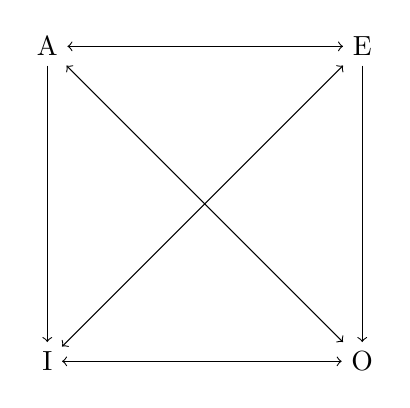
\begin{tikzpicture}
  \node(A) at (0,0) {A};
  \node(E) at (4,0) {E};
  \node(I) at (0,-4) {I};
  \node(O) at (4,-4) {O};
  \draw[<->] (A) -- (E);
  \draw[<->] (I) -- (O);
  \draw[<->] (A) -- (O);
  \draw[<->] (E) -- (I);
  \draw[->] (A) -- (I);
  \draw[->] (E) -- (O);
\end{tikzpicture}

The next step is to note the relationship between the diagonals. The diagonals are contradictories, meaning they always have opposite truth values. They can't both be true, and they also can't both be false.  If the A sentence is true, the O sentence must be false---if it is true that all dogs are mammals, it cannot be true that some dogs are not mammals. If the O sentence is true, then the A sentence must be false. It is the same for the E and the I. 

\medskip
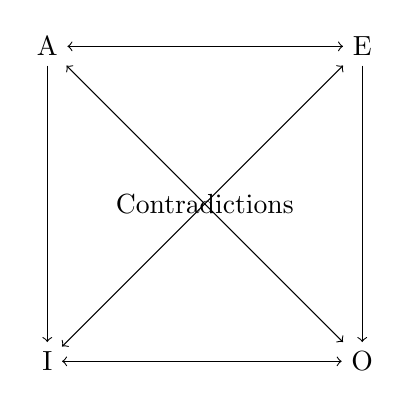
\begin{tikzpicture}
  \node(A) at (0,0) {A};
  \node(E) at (4,0) {E};
  \node(I) at (0,-4) {I};
  \node(O) at (4,-4) {O};
  \draw[<->] (A) -- (E);
  \draw[<->] (I) -- (O);
  \draw[<->] (A) -- (O) node[pos=0.5]{Contradictions};
  \draw[<->] (E) -- (I);
  \draw[->] (A) -- (I);
  \draw[->] (E) -- (O);
  % \draw (-0.5,0) node[left]{Altern};
  % \draw (4.5,0) node[right]{Altern};
  % \draw (-0.5,-4) node[left]{Sub-altern};
  % \draw (4.5,-4) node[right]{Sub-altern};
\end{tikzpicture}

Next, note the relationship between the A sentences and the E sentences, called contraries. Like the contradictories, they cannot both be true. Unlike the contradictories, they can both be false. If it's true that all critical thinking students are good students, then it must be false that no critical thinking students are good students. If it's false that all critical thinking students are good students, then it can be false that critical thinking students are good students. In fact, they are both false, because some critical thinking students are good and others are not. 

\medskip
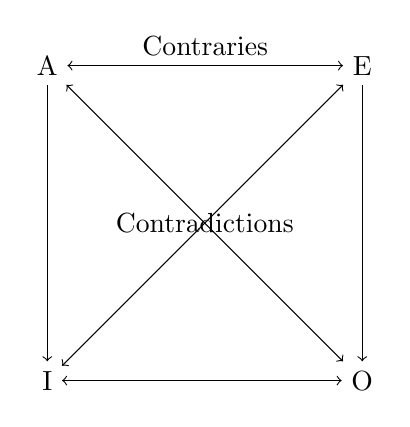
\begin{tikzpicture}
  \node(A) at (0,0) {A};
  \node(E) at (4,0) {E};
  \node(I) at (0,-4) {I};
  \node(O) at (4,-4) {O};
  \draw[<->] (A) -- (E) node[pos=0.5,anchor=south]{Contraries};
  \draw[<->] (I) -- (O);
  \draw[<->] (A) -- (O) node[pos=0.5]{Contradictions};
  \draw[<->] (E) -- (I);
  \draw[->] (A) -- (I);
  \draw[->] (E) -- (O);
  % \draw (-0.5,0) node[left]{Altern};
  % \draw (4.5,0) node[right]{Altern};
  % \draw (-0.5,-4) node[left]{Sub-altern};
  % \draw (4.5,-4) node[right]{Sub-altern};
\end{tikzpicture}

At the bottom, we have sub-contraries. They can both be false, but cannot both be true.

\medskip
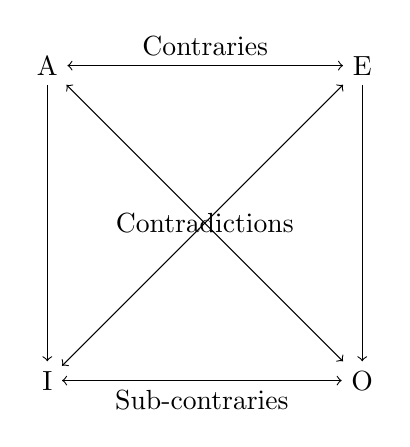
\begin{tikzpicture}
  \node(A) at (0,0) {A};
  \node(E) at (4,0) {E};
  \node(I) at (0,-4) {I};
  \node(O) at (4,-4) {O};
  \draw[<->] (A) -- (E) node[pos=0.5,anchor=south]{Contraries};
  \draw[<->] (I) -- (O)node[pos=0.5,anchor=north]{Sub-contraries};
  \draw[<->] (A) -- (O) node[pos=0.5]{Contradictions};
  \draw[<->] (E) -- (I);
  \draw[->] (A) -- (I);
  \draw[->] (E) -- (O);
  % \draw (-0.5,0) node[left]{Altern};
  % \draw (4.5,0) node[right]{Altern};
  % \draw (-0.5,-4) node[left]{Sub-altern};
  % \draw (4.5,-4) node[right]{Sub-altern};
\end{tikzpicture}

Finally, we have the relationship between the top level sentences and the bottom level sentences on the same side. This is called alternation. The universal is called the superaltern and the particular is called the subaltern. If the superaltern is true, then the subaltern must also be true. If the superaltern is false, then the subaltern can be either true or false. If the subaltern is false, then the superaltern must be false. If the subaltern is true, then the superaltern can be either true or false. It is easy to remember this way: truth goes down, falsity goes up.

\medskip
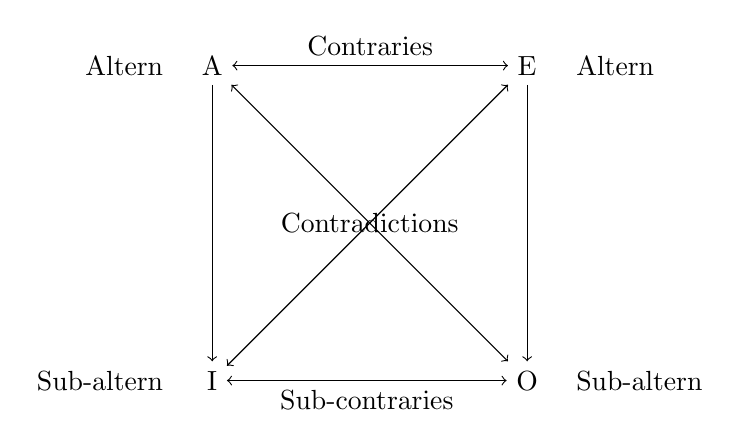
\begin{tikzpicture}
  \node(A) at (0,0) {A};
  \node(E) at (4,0) {E};
  \node(I) at (0,-4) {I};
  \node(O) at (4,-4) {O};
  \draw[<->] (A) -- (E) node[pos=0.5,anchor=south]{Contraries};
  \draw[<->] (I) -- (O)node[pos=0.5,anchor=north]{Sub-contraries};
  \draw[<->] (A) -- (O) node[pos=0.5]{Contradictions};
  \draw[<->] (E) -- (I);
  \draw[->] (A) -- (I);
  \draw[->] (E) -- (O);
  \draw (-0.5,0) node[left]{Altern};
  \draw (4.5,0) node[right]{Altern};
  \draw (-0.5,-4) node[left]{Sub-altern};
  \draw (4.5,-4) node[right]{Sub-altern};
\end{tikzpicture}

\section{Diagramming Sentences}
\label{sec:diagramming-sentences}



We diagram sentences and arguments in categorical logic using Venn diagrams. You've probably used these in a math class at some time. Before we can use these to evaluate arguments in categorical logic, we first have to learn how to diagram individual sentences.

The first step is to draw two interlocking circles. Label the left circle with an \enquote{S} and the right circle with \enquote{P}---standing for the subject term and predicate term, respectively.

\def\sub{(0,0) circle (1.5cm)}
\def\mid{(-60:2cm) circle (1.5cm)}
\def\pred{(0:2cm) circle (1.5cm)}

\medskip
\begin{tikzpicture}[thick,scale=1, every node/.style={transform shape}]
  \begin{scope}
    % A-Sentences

    % \begin{scope}[even odd rule]% Shade S without P
    %   \clip \pred (-1.5,-1.5) rectangle (1.5,1.5);
    %   \fill[gray] \sub;
    % \end{scope}

    % \begin{scope}[even odd rule]% Shade S without M
    %   \clip \mid (-1.5,-1.5) rectangle (1.5,1.5);
    %   \fill[gray] \sub;
    % \end{scope}

    % \begin{scope}[even odd rule]% Shade M without S
    %   \clip \sub (-0.5,-3.3) rectangle (2.5,0);
    %   \fill[gray] \mid;
    % \end{scope}

    % \begin{scope}[even odd rule]% Shade M without P
    %   \clip \pred (-0.5,-3.3) rectangle (2.5,0);
    %   \fill[gray] \mid;
    % \end{scope}

    % \begin{scope}[even odd rule]% Shade P without M
    %   \clip \mid (-0,-1.5) rectangle (3.5,1.5);
    %   \fill[gray] \pred;
    % \end{scope}

    % \begin{scope}[even odd rule]% Shade P without S
    %   \clip \sub (0,-1.5) rectangle (3.5,1.5);
    %   \fill[gray] \pred;
    % \end{scope}

    % E Sentences

    % \begin{scope} %Shade intersection of S and P
    %   \clip \pred;
    %   \fill[gray] \sub;
    % \end{scope}

    % \begin{scope} %Shade intersection of S and M
    %   \clip \mid;
    %   \fill[gray] \sub;
    % \end{scope}

    % \begin{scope} %Shade intersection of M and P
    %   \clip \pred;
    %   \fill[gray] \mid;
    % \end{scope}

    % Mark I and O Sentences

    % \draw (-0.5,0.3) node {1};
    % \draw (1,0.3) node {2};
    % \draw (2.5,0.3) node {3};
    % \draw (0.2,-0.9) node {4};
    % \draw (1,-0.6) node {5};
    % \draw (1.8,-0.9) node {6};
    % \draw (1,-2) node {7};

    % Label Circles

    \draw (-2,-0) node {$S$};
    % \draw (1,-4) node {$M$};
    \draw (4,0) node {$P$};

    % Draw Circles

    \draw \sub;
    \draw \pred;
    % \draw \mid;
  \end{scope}

\end{tikzpicture}

\subsection{A-Sentences}

Remember that the A-sentence has the form All S are P. That means that everything that is in the S circle must also be in the P circle. To diagram this, we shade the region of the S circle that is not contained in the P circle. If a region is shaded, that means that nothing is in that region.



\medskip
\begin{tikzpicture}[thick,scale=1, every node/.style={transform shape}]
  \begin{scope}
    % A-Sentences

    \begin{scope}[even odd rule]% Shade S without P
      \clip \pred (-1.5,-1.5) rectangle (1.5,1.5);
      \fill[gray] \sub;
    \end{scope}

    % \begin{scope}[even odd rule]% Shade S without M
    %   \clip \mid (-1.5,-1.5) rectangle (1.5,1.5);
    %   \fill[gray] \sub;
    % \end{scope}

    % \begin{scope}[even odd rule]% Shade M without S
    %   \clip \sub (-0.5,-3.3) rectangle (2.5,0);
    %   \fill[gray] \mid;
    % \end{scope}

    % \begin{scope}[even odd rule]% Shade M without P
    %   \clip \pred (-0.5,-3.3) rectangle (2.5,0);
    %   \fill[gray] \mid;
    % \end{scope}

    % \begin{scope}[even odd rule]% Shade P without M
    %   \clip \mid (-0,-1.5) rectangle (3.5,1.5);
    %   \fill[gray] \pred;
    % \end{scope}

    % \begin{scope}[even odd rule]% Shade P without S
    %   \clip \sub (0,-1.5) rectangle (3.5,1.5);
    %   \fill[gray] \pred;
    % \end{scope}

    % E Sentences

    % \begin{scope} %Shade intersection of S and P
    %   \clip \pred;
    %   \fill[gray] \sub;
    % \end{scope}

    % \begin{scope} %Shade intersection of S and M
    %   \clip \mid;
    %   \fill[gray] \sub;
    % \end{scope}

    % \begin{scope} %Shade intersection of M and P
    %   \clip \pred;
    %   \fill[gray] \mid;
    % \end{scope}

    % Mark I and O Sentences

    % \draw (-0.5,0.3) node {1};
    % \draw (1,0.3) node {2};
    % \draw (2.5,0.3) node {3};
    % \draw (0.2,-0.9) node {4};
    % \draw (1,-0.6) node {5};
    % \draw (1.8,-0.9) node {6};
    % \draw (1,-2) node {7};

    % Label Circles

    \draw (-2,-0) node {$S$};
    % \draw (1,-4) node {$M$};
    \draw (4,0) node {$P$};

    % Draw Circles

    \draw \sub;
    \draw \pred;
    % \draw \mid;
  \end{scope}

\end{tikzpicture}

\subsection{E-Sentences}

To shade the universal negation, we shade the region that is shared by both S and P:


\medskip
\begin{tikzpicture}[thick,scale=1, every node/.style={transform shape}]
  \begin{scope}
    % A-Sentences

    % \begin{scope}[even odd rule]% Shade S without P
    %   \clip \pred (-1.5,-1.5) rectangle (1.5,1.5);
    %   \fill[gray] \sub;
    % \end{scope}

    % \begin{scope}[even odd rule]% Shade S without M
    %   \clip \mid (-1.5,-1.5) rectangle (1.5,1.5);
    %   \fill[gray] \sub;
    % \end{scope}

    % \begin{scope}[even odd rule]% Shade M without S
    %   \clip \sub (-0.5,-3.3) rectangle (2.5,0);
    %   \fill[gray] \mid;
    % \end{scope}

    % \begin{scope}[even odd rule]% Shade M without P
    %   \clip \pred (-0.5,-3.3) rectangle (2.5,0);
    %   \fill[gray] \mid;
    % \end{scope}

    % \begin{scope}[even odd rule]% Shade P without M
    %   \clip \mid (-0,-1.5) rectangle (3.5,1.5);
    %   \fill[gray] \pred;
    % \end{scope}

    % \begin{scope}[even odd rule]% Shade P without S
    %   \clip \sub (0,-1.5) rectangle (3.5,1.5);
    %   \fill[gray] \pred;
    % \end{scope}

    % E Sentences

    \begin{scope} %Shade intersection of S and P
      \clip \pred;
      \fill[gray] \sub;
    \end{scope}

    % \begin{scope} %Shade intersection of S and M
    %   \clip \mid;
    %   \fill[gray] \sub;
    % \end{scope}

    % \begin{scope} %Shade intersection of M and P
    %   \clip \pred;
    %   \fill[gray] \mid;
    % \end{scope}

    % Mark I and O Sentences

    % \draw (-0.5,0.3) node {1};
    % \draw (1,0.3) node {2};
    % \draw (2.5,0.3) node {3};
    % \draw (0.2,-0.9) node {4};
    % \draw (1,-0.6) node {5};
    % \draw (1.8,-0.9) node {6};
    % \draw (1,-2) node {7};

    % Label Circles

    \draw (-2,-0) node {$S$};
    % \draw (1,-4) node {$M$};
    \draw (4,0) node {$P$};

    % Draw Circles

    \draw \sub;
    \draw \pred;
    % \draw \mid;
  \end{scope}

\end{tikzpicture}

\subsection{I-Sentences}

To diagram a particular affirmation, we place an x in the region shared by S and P:



\medskip
\begin{tikzpicture}[thick,scale=1, every node/.style={transform shape}]
  \begin{scope}
    % A-Sentences

    % \begin{scope}[even odd rule]% Shade S without P
    %   \clip \pred (-1.5,-1.5) rectangle (1.5,1.5);
    %   \fill[gray] \sub;
    % \end{scope}

    % \begin{scope}[even odd rule]% Shade S without M
    %   \clip \mid (-1.5,-1.5) rectangle (1.5,1.5);
    %   \fill[gray] \sub;
    % \end{scope}

    % \begin{scope}[even odd rule]% Shade M without S
    %   \clip \sub (-0.5,-3.3) rectangle (2.5,0);
    %   \fill[gray] \mid;
    % \end{scope}

    % \begin{scope}[even odd rule]% Shade M without P
    %   \clip \pred (-0.5,-3.3) rectangle (2.5,0);
    %   \fill[gray] \mid;
    % \end{scope}

    % \begin{scope}[even odd rule]% Shade P without M
    %   \clip \mid (-0,-1.5) rectangle (3.5,1.5);
    %   \fill[gray] \pred;
    % \end{scope}

    % \begin{scope}[even odd rule]% Shade P without S
    %   \clip \sub (0,-1.5) rectangle (3.5,1.5);
    %   \fill[gray] \pred;
    % \end{scope}

    % E Sentences

    % \begin{scope} %Shade intersection of S and P
    %   \clip \pred;
    %   \fill[gray] \sub;
    % \end{scope}

    % \begin{scope} %Shade intersection of S and M
    %   \clip \mid;
    %   \fill[gray] \sub;
    % \end{scope}

    % \begin{scope} %Shade intersection of M and P
    %   \clip \pred;
    %   \fill[gray] \mid;
    % \end{scope}

    % Mark I and O Sentences

    % \draw (-0.5,0.3) node {1};
    % \draw (1,0.3) node {2};
    \draw (1,0) node {x};
    % \draw (2.5,0.3) node {3};
    % \draw (0.2,-0.9) node {4};
    % \draw (1,-0.6) node {5};
    % \draw (1.8,-0.9) node {6};
    % \draw (1,-2) node {7};

    % Label Circles

    \draw (-2,-0) node {$S$};
    % \draw (1,-4) node {$M$};
    \draw (4,0) node {$P$};

    % Draw Circles

    \draw \sub;
    \draw \pred;
    % \draw \mid;
  \end{scope}

\end{tikzpicture}


\subsection{O-Sentences}

Finally, to diagram an O-sentence, we place an x in S, but not in P:



\medskip
\begin{tikzpicture}[thick,scale=1, every node/.style={transform shape}]
  \begin{scope}
    % A-Sentences

    % \begin{scope}[even odd rule]% Shade S without P
    %   \clip \pred (-1.5,-1.5) rectangle (1.5,1.5);
    %   \fill[gray] \sub;
    % \end{scope}

    % \begin{scope}[even odd rule]% Shade S without M
    %   \clip \mid (-1.5,-1.5) rectangle (1.5,1.5);
    %   \fill[gray] \sub;
    % \end{scope}

    % \begin{scope}[even odd rule]% Shade M without S
    %   \clip \sub (-0.5,-3.3) rectangle (2.5,0);
    %   \fill[gray] \mid;
    % \end{scope}

    % \begin{scope}[even odd rule]% Shade M without P
    %   \clip \pred (-0.5,-3.3) rectangle (2.5,0);
    %   \fill[gray] \mid;
    % \end{scope}

    % \begin{scope}[even odd rule]% Shade P without M
    %   \clip \mid (-0,-1.5) rectangle (3.5,1.5);
    %   \fill[gray] \pred;
    % \end{scope}

    % \begin{scope}[even odd rule]% Shade P without S
    %   \clip \sub (0,-1.5) rectangle (3.5,1.5);
    %   \fill[gray] \pred;
    % \end{scope}

    % E Sentences

    % \begin{scope} %Shade intersection of S and P
    %   \clip \pred;
    %   \fill[gray] \sub;
    % \end{scope}

    % \begin{scope} %Shade intersection of S and M
    %   \clip \mid;
    %   \fill[gray] \sub;
    % \end{scope}

    % \begin{scope} %Shade intersection of M and P
    %   \clip \pred;
    %   \fill[gray] \mid;
    % \end{scope}

    % Mark I and O Sentences

    \draw (-0.5,0) node {x};
    

    % Label Circles

    \draw (-2,-0) node {$S$};
    % \draw (1,-4) node {$M$};
    \draw (4,0) node {$P$};

    % Draw Circles

    \draw \sub;
    \draw \pred;
    % \draw \mid;
  \end{scope}

\end{tikzpicture}




\subsection{Evaluating Categorical Syllogisms}

A syllogism is an argument that has two premises and a conclusion. A categorical syllogism is a syllogism that contains only categorical sentences. Here is an example:

\begin{enumerate}
\item All Dogs are mammals.
\item \underline{All mammals are animals.}
\item [$\therefore$]All dogs are animals
\end{enumerate}

Both premises and the conclusion are A-sentences. Notice that we have three terms in the argument: dogs, mammals, and animals. Every categorical syllogism, in proper form, has three terms. Each term occurs in two sentences. Two of those terms will be found in the conclusion, and one term is only in the premises. The predicate term of the conclusion is called the major term. The subject of the conclusion is called the minor term. The term that is not in the conclusion is called the middle term.

There are two ways to determine if a categorical syllogism is valid. One way uses Venn diagrams, and the other involves applying some simple rules.

\subsection{Diagram Method}

Since we have three terms in the argument, we'll need three intersecting circles. We'll start by drawing two circles for the conclusion, just as we did before. Then, in the middle and below, we'll draw another circle for the middle term. For labels, use letters that correspond to the classes in the argument. Here, we'll use D for dogs, M for mammals, and A for animals.


\medskip
\begin{tikzpicture}[thick,scale=1, every node/.style={transform shape}]
  \begin{scope}
    % A-Sentences

    % \begin{scope}[even odd rule]% Shade S without P
    %   \clip \pred (-1.5,-1.5) rectangle (1.5,1.5);
    %   \fill[gray] \sub;
    % \end{scope}

    % \begin{scope}[even odd rule]% Shade S without M
    %   \clip \mid (-1.5,-1.5) rectangle (1.5,1.5);
    %   \fill[gray] \sub;
    % \end{scope}

    % \begin{scope}[even odd rule]% Shade M without S
    %   \clip \sub (-0.5,-3.3) rectangle (2.5,0);
    %   \fill[gray] \mid;
    % \end{scope}

    % \begin{scope}[even odd rule]% Shade M without P
    %   \clip \pred (-0.5,-3.3) rectangle (2.5,0);
    %   \fill[gray] \mid;
    % \end{scope}

    % \begin{scope}[even odd rule]% Shade P without M
    %   \clip \mid (-0,-1.5) rectangle (3.5,1.5);
    %   \fill[gray] \pred;
    % \end{scope}

    % \begin{scope}[even odd rule]% Shade P without S
    %   \clip \sub (0,-1.5) rectangle (3.5,1.5);
    %   \fill[gray] \pred;
    % \end{scope}

    % E Sentences

    % \begin{scope} %Shade intersection of S and P
    %   \clip \pred;
    %   \fill[gray] \sub;
    % \end{scope}

    % \begin{scope} %Shade intersection of S and M
    %   \clip \mid;
    %   \fill[gray] \sub;
    % \end{scope}

    % \begin{scope} %Shade intersection of M and P
    %   \clip \pred;
    %   \fill[gray] \mid;
    % \end{scope}

    % Mark I and O Sentences

    % \draw (-0.5,0.3) node {1};
    % \draw (1,0.3) node {2};
    % \draw (2.5,0.3) node {3};
    % \draw (0.2,-0.9) node {4};
    % \draw (1,-0.6) node {5};
    % \draw (1.8,-0.9) node {6};
    % \draw (1,-2) node {7};

    % Label Circles

    \draw (-2,-0) node {$D$};
    \draw (1,-4) node {$M$};
    \draw (4,0) node {$A$};

    % Draw Circles

    \draw \sub;
    \draw \pred;
    \draw \mid;
  \end{scope}

\end{tikzpicture}



Next, we finish diagramming the premises by shading or placing an x. Since our first premise is \enquote{All dogs are mammals}, we need to shade everything in the D circle that is not in the M circle.


\medskip
\begin{tikzpicture}[thick,scale=1, every node/.style={transform shape}]
  \begin{scope}
    % A-Sentences

    % \begin{scope}[even odd rule]% Shade S without P
    %   \clip \pred (-1.5,-1.5) rectangle (1.5,1.5);
    %   \fill[gray] \sub;
    % \end{scope}

    \begin{scope}[even odd rule]% Shade S without M
      \clip \mid (-1.5,-1.5) rectangle (1.5,1.5);
      \fill[gray] \sub;
    \end{scope}

    % \begin{scope}[even odd rule]% Shade M without S
    %   \clip \sub (-0.5,-3.3) rectangle (2.5,0);
    %   \fill[gray] \mid;
    % \end{scope}

    % \begin{scope}[even odd rule]% Shade M without P
    %   \clip \pred (-0.5,-3.3) rectangle (2.5,0);
    %   \fill[gray] \mid;
    % \end{scope}

    % \begin{scope}[even odd rule]% Shade P without M
    %   \clip \mid (-0,-1.5) rectangle (3.5,1.5);
    %   \fill[gray] \pred;
    % \end{scope}

    % \begin{scope}[even odd rule]% Shade P without S
    %   \clip \sub (0,-1.5) rectangle (3.5,1.5);
    %   \fill[gray] \pred;
    % \end{scope}

    % E Sentences

    % \begin{scope} %Shade intersection of S and P
    %   \clip \pred;
    %   \fill[gray] \sub;
    % \end{scope}

    % \begin{scope} %Shade intersection of S and M
    %   \clip \mid;
    %   \fill[gray] \sub;
    % \end{scope}

    % \begin{scope} %Shade intersection of M and P
    %   \clip \pred;
    %   \fill[gray] \mid;
    % \end{scope}

    % Mark I and O Sentences

    % \draw (-0.5,0.3) node {1};
    % \draw (1,0.3) node {2};
    % \draw (2.5,0.3) node {3};
    % \draw (0.2,-0.9) node {4};
    % \draw (1,-0.6) node {5};
    % \draw (1.8,-0.9) node {6};
    % \draw (1,-2) node {7};

    % Label Circles

    \draw (-2,-0) node {$D$};
    \draw (1,-4) node {$M$};
    \draw (4,0) node {$A$};

    % Draw Circles

    \draw \sub;
    \draw \pred;
    \draw \mid;
  \end{scope}

\end{tikzpicture}



Next, we diagram the second premise by shading everything that is in the M circle but not in the A circle.

\medskip
\begin{tikzpicture}[thick,scale=1, every node/.style={transform shape}]
  \begin{scope}
    % A-Sentences

    % \begin{scope}[even odd rule]% Shade S without P
    %   \clip \pred (-1.5,-1.5) rectangle (1.5,1.5);
    %   \fill[gray] \sub;
    % \end{scope}

    \begin{scope}[even odd rule]% Shade S without M
      \clip \mid (-1.5,-1.5) rectangle (1.5,1.5);
      \fill[gray] \sub;
    \end{scope}

    % \begin{scope}[even odd rule]% Shade M without S
    %   \clip \sub (-0.5,-3.3) rectangle (2.5,0);
    %   \fill[gray] \mid;
    % \end{scope}

    \begin{scope}[even odd rule]% Shade M without P
      \clip \pred (-0.5,-3.3) rectangle (2.5,0);
      \fill[gray] \mid;
    \end{scope}

    % \begin{scope}[even odd rule]% Shade P without M
    %   \clip \mid (-0,-1.5) rectangle (3.5,1.5);
    %   \fill[gray] \pred;
    % \end{scope}

    % \begin{scope}[even odd rule]% Shade P without S
    %   \clip \sub (0,-1.5) rectangle (3.5,1.5);
    %   \fill[gray] \pred;
    % \end{scope}

    % E Sentences

    % \begin{scope} %Shade intersection of S and P
    %   \clip \pred;
    %   \fill[gray] \sub;
    % \end{scope}

    % \begin{scope} %Shade intersection of S and M
    %   \clip \mid;
    %   \fill[gray] \sub;
    % \end{scope}

    % \begin{scope} %Shade intersection of M and P
    %   \clip \pred;
    %   \fill[gray] \mid;
    % \end{scope}

    % Mark I and O Sentences

    % \draw (-0.5,0.3) node {1};
    % \draw (1,0.3) node {2};
    % \draw (2.5,0.3) node {3};
    % \draw (0.2,-0.9) node {4};
    % \draw (1,-0.6) node {5};
    % \draw (1.8,-0.9) node {6};
    % \draw (1,-2) node {7};

    % Label Circles

    \draw (-2,-0) node {$D$};
    \draw (1,-4) node {$M$};
    \draw (4,0) node {$A$};

    % Draw Circles

    \draw \sub;
    \draw \pred;
    \draw \mid;
  \end{scope}

\end{tikzpicture}




If there is any circle that has only one region left unshaded, you can place an `X' in that region. This is because categorical logic assumes that there are no empty categories, meaning that every category has at least one thing in it. This is really only important for arguments that have an I or an O-sentence for a conclusion. In this case, we won't worry about it.  Now that the premises are diagrammed, check to see if the conclusion has also been diagrammed, which in this case means that everything in the D circle that is not also in the A circle is shaded out. If so, then the argument is valid. This shows that making the premises true was enough to make the conclusion true also.

Let's try to diagram this argument:

\begin{enumerate}
\item No introverts are politicians 
\item \underline{All artists are introverts}
\item No artists are politicians
\end{enumerate}

% \medskip
% \begin{tikzpicture}[thick,scale=1, every node/.style={transform shape}]
%   \begin{scope}
%     % A-Sentences
%     \begin{scope}[even odd rule]% Shade S without M
%       \clip \mid (-1.5,-1.5) rectangle (1.5,1.5);
%       \fill[gray] \sub;
%     \end{scope}

%     % E Sentences
%     \begin{scope} %Shade intersection of M and P
%       \clip \pred;
%       \fill[gray] \mid;
%     \end{scope}

%     % Label Circles
%     \draw (-2,-0) node {$A$};
%     \draw (1,-4) node {$I$};
%     \draw (4,0) node {$P$};

%     % Draw Circles
%     \draw \sub;
%     \draw \pred;
%     \draw \mid;
%   \end{scope}
% \end{tikzpicture}

First, we draw and label the circles:

\medskip
\begin{tikzpicture}[thick,scale=1, every node/.style={transform shape}]
  \begin{scope}
    % A-Sentences
    % \begin{scope}[even odd rule]% Shade S without M
    %   \clip \mid (-1.5,-1.5) rectangle (1.5,1.5);
    %   \fill[gray] \sub;
    % \end{scope}

    % % E Sentences
    % \begin{scope} %Shade intersection of M and P
    %   \clip \pred;
    %   \fill[gray] \mid;
    % \end{scope}

    % Label Circles
    \draw (-2,-0) node {$A$};
    \draw (1,-4) node {$I$};
    \draw (4,0) node {$P$};

    % Draw Circles
    \draw \sub;
    \draw \pred;
    \draw \mid;
  \end{scope}

\end{tikzpicture}

Then we diagram the premises, always doing the universals before any particulars. In this case, we have two universal premises, so we will just begin with the first premise:

\medskip
\begin{tikzpicture}[thick,scale=1, every node/.style={transform shape}]
  \begin{scope}
    % A-Sentences
    % \begin{scope}[even odd rule]% Shade S without M
    %   \clip \mid (-1.5,-1.5) rectangle (1.5,1.5);
    %   \fill[gray] \sub;
    % \end{scope}

    % E Sentences
    \begin{scope} %Shade intersection of M and P
      \clip \pred;
      \fill[gray] \mid;
    \end{scope}

    % Label Circles
    \draw (-2,-0) node {$A$};
    \draw (1,-4) node {$I$};
    \draw (4,0) node {$P$};

    % Draw Circles
    \draw \sub;
    \draw \pred;
    \draw \mid;
  \end{scope}

\end{tikzpicture}

Now, we'll diagram the second premise:

\medskip
\begin{tikzpicture}[thick,scale=1, every node/.style={transform shape}]
  \begin{scope}
    % A-Sentences
    \begin{scope}[even odd rule]% Shade S without M
      \clip \mid (-1.5,-1.5) rectangle (1.5,1.5);
      \fill[gray] \sub;
    \end{scope}

    % E Sentences
    \begin{scope} %Shade intersection of M and P
      \clip \pred;
      \fill[gray] \mid;
    \end{scope}

    % Label Circles
    \draw (-2,-0) node {$A$};
    \draw (1,-4) node {$I$};
    \draw (4,0) node {$P$};

    % Draw Circles
    \draw \sub;
    \draw \pred;
    \draw \mid;
  \end{scope}

\end{tikzpicture}

Diagramming the conclusion would require the intersection of $A$ and $P$ to be shaded. Notice, though, that the region between $A$ and $P$ has already been shaded by just diagramming the premises. That means that making the premises true was enough to guarantee that the conclusion would also be true, and the argument is valid.


Let's try one more argument.

\begin{enumerate}
\item Some horses are things that weigh over 2,000 pounds.
\item \underline{All horses are mammals.}
\item Some mammals are things that weigh over 2,000 pounds.
\end{enumerate}

Again, we begin by drawing and labeling the circles.

\medskip
\begin{tikzpicture}[thick,scale=1, every node/.style={transform shape}]
  \begin{scope}
    % A-Sentences


    % \begin{scope}[even odd rule]% Shade M without S
    %   \clip \sub (-0.5,-3.3) rectangle (2.5,0);
    %   \fill[gray] \mid;
    % \end{scope}

    % Mark I and O Sentences
    % \draw (1,-0.6) node {x};
    
    % Label Circles
    \draw (-2,-0) node {$M$};
    \draw (1,-4) node {$H$};
    \draw (4,0) node {$W$};

    % Draw Circles
    \draw \sub;
    \draw \pred;
    \draw \mid;
  \end{scope}

\end{tikzpicture}


The we diagram any universal premises, which, in this case, is the second premise.


\medskip
\begin{tikzpicture}[thick,scale=1, every node/.style={transform shape}]
  \begin{scope}
    % A-Sentences


    \begin{scope}[even odd rule]% Shade M without S
      \clip \sub (-0.5,-3.3) rectangle (2.5,0);
      \fill[gray] \mid;
    \end{scope}

    % Mark I and O Sentences
    % \draw (1,-0.6) node {x};
    
    % Label Circles
    \draw (-2,-0) node {$M$};
    \draw (1,-4) node {$H$};
    \draw (4,0) node {$W$};

    % Draw Circles
    \draw \sub;
    \draw \pred;
    \draw \mid;
  \end{scope}

\end{tikzpicture}

Then, we diagram any particular premises.


\medskip
\begin{tikzpicture}[thick,scale=1, every node/.style={transform shape}]
  \begin{scope}
    % A-Sentences


    \begin{scope}[even odd rule]% Shade M without S
      \clip \sub (-0.5,-3.3) rectangle (2.5,0);
      \fill[gray] \mid;
    \end{scope}

    % Mark I and O Sentences
    \draw (1,-0.6) node {x};
    
    % Label Circles
    \draw (-2,-0) node {$M$};
    \draw (1,-4) node {$H$};
    \draw (4,0) node {$W$};

    % Draw Circles
    \draw \sub;
    \draw \pred;
    \draw \mid;
  \end{scope}

\end{tikzpicture}

Finally, we check to see if diagramming the premises was enough to make the conclusion also diagrammed. In this case, it was, so the argument is valid.


\subsection{Hints for Diagramming Categorical Syllogisms}

\begin{enumerate}

  

\item Diagram universals before particulars (shade before making an x.)
\item If it is not clear where the x goes, then put it on the line.
\end{enumerate}

\section{Rules for Categorical Syllogisms}

There is another way to determine validity for categorical syllogisms. Every valid syllogism must meet three conditions:


\begin{enumerate}


\item There must be the same number of negations in the conclusion as in the premises.
\item The middle term must be distributed at least once.
\item Any term distributed in the conclusion must be distributed in the premises.
\end{enumerate}

Before these rules can be applied, we'll have to explain what distribution is. Every categorical statement says something about a category or class. A statement distributes a term just in case what it says about that class is true of every subset of the class. For example, it is true that all dogs are mammals. It's also true that all members of any subset of the set of dogs are mammals---all dogs in Oklahoma are mammals, and all dogs in Greece are mammals, and so on. All dogs are not necessarily members of every subset of the class of mammals, however. The class of cats is a subset of the class of mammals, and no dog is a cat. So, the subject of an A-sentence is distributed, but the predicate is not.  To remember when something is distributed, keep this in mind:

\begin{enumerate}
\item Universals distribute subjects, and
\item Negations distribute predicates.
\end{enumerate}

So, A-sentences distribute the subject, E-sentences distribute both terms, I-sentences don't distribute anything, and O sentences distribute the predicate.

The rules are easy to apply. First, put the argument in standard form:

\begin{enumerate}
  % \tightlist
\item All A are B.
\item \underline{All B are C.}
\item [$\therefore$] All A are C.
\end{enumerate}

Then, circle all of the distributed terms.

\begin{enumerate}
  % \tightlist
\item All \textcircled{A} are B.
\item \underline{All \textcircled{B} are C.}
\item [$\therefore$] All \textcircled{A} are C.
\end{enumerate}

Now, just check to see if there are any violations of the rules:

\begin{enumerate}
\item Are there the same number of negations in the conclusion as in the premises? Yes, since there are no negations at all.
\item Is the middle term distributed at least once? Yes, the middle term is B and it is distributed in the second premise.
\item Is any term that distributed in the conclusion also distributed in the premises? Yes, A is distributed in the conclusion, but it is also distributed in the first premise.
\end{enumerate}


So, since the argument breaks none of the rules, it is valid.



\section{Relations of Equivalence}

Properly formed categorical syllogisms have only three terms. Unfortunately, some arguments that you will encounter won't always be in proper form. One common way this happens is for a person to use a term like \enquote{Americans} in one premise, but use \enquote{non-Americans} in another. This can result in a syllogism with four or more terms, making it impossible to evaluate using either of our two methods. What we then need to do is to convert the sentence using one of the terms into a logically equivalent sentence that uses the other term.


There are three operations that can be applied to categorical sentences: conversion, obversion, and contraposition. It is important to know both how to apply them and in what cases does an operation result in an equivalent sentence. We're particularly interested in the conditions that those different operations are *truth-preserving*. An operation is truth preserving when, applied to a true sentence, it always results in a true sentence.

\subsection{Conversion}


Conversion is the simplest of the three. The converse of a sentence simply exchanges the subject and predicate terms of the original sentence. Conversion applied to A-sentences is \emph{not} truth-preserving. \enquote{All dogs are mammals} is true, but \enquote{All mammals are dogs} is not. Conversion is truth-preserving for E-sentences and I-sentences. If it is true that no dogs are reptiles, it must be true that no reptiles are dots. Likewise, if it is true that some dogs are brown things, it must be true that some brown things are dogs.

Another way to think about this is to consider what the diagrams would like before the change and after the change. Before the change, the diagram looks like figure below, with the intersection of the S and P circles shaded.

After the change, the diagram looks like figure , with the intersection of the S and P circles shaded. Essentially, there's been no change. Imagine what it would like to view the first diagram from behind, or upside-down. In either case, what you would see is the same as the first diagram.


\subsection{Obversion}

Take another look at the square of opposition in figure 4.1. Note that the A and the E are straight across from each other, as are the I and the O. The first step in forming the obverse is to first change the sentence into the type that is straight across the square of opposition. That is, if you started with an A-sentence, then make it into and E. The O becomes and I, and so on.


Once you've changed the sentence type, the next step is to change predicate into its complement. The complement of a class $C$ is the class of everything that is not in $C$. The easiest way to form a complement is to prefix the class with `non'. For example, the complement of the class of students is the class of non-students.

So, the obverse of all dogs are mammals is no dogs are non-mammals. The obverse of no OBU students are martians is all OBU students are non-martians. Obversion is truth-preserving in all cases.

\subsection{Contraposition}

The last of our three relations is contraposition. To form the contrapositive of a sentence, first form the converse, then exchange both terms for their complements.

The contrapositive of all dogs are mammals is all non-mammals are non-dogs. Contraposition is truth-preserving for A-sentences and O-sentences only.

\newpage

Here's a table to help keep this straight (operations that are truth-preserving are in bold type):


% Please add the following required packages to your document preamble:
% \usepackage{booktabs}
\begin{table}[]
\begin{tabular}{@{}llll@{}}
\toprule
Original         & Converse         & Obverse              & Contrapositive           \\ \midrule
All S are P      & All P are S      & \textbf{No S are non-P}       & \textbf{All non-P are non-S}      \\
No S are P       & \textbf{No P are S}       & \textbf{All S are non-P}      & No non-P are non-S       \\
Some S are P     & \textbf{Some P are S}     & \textbf{Some S are not non-P} & Some non-P are non-S     \\
Some S are not P & Some P are not S & \textbf{Some S are non-P}     & \textbf{Some non-P are not non-S} \\ \bottomrule
\end{tabular}
\end{table}

\subsection{Example}

Look at the following argument:

\begin{enumerate}
\item All Catholics are non-Protestants.
\item \underline{All Lutherans are Protestants.}
\item No Catholics are Lutherans.
\end{enumerate}

Note that this argument has four terms:

\begin{enumerate}

\item Catholics
\item Non-Protestants
\item Lutherans
\item Protestants

\end{enumerate}

To evaluate the argument, we will first have to either change \enquote{non-Protestants} to \enquote{Protestants} in the first premise, or \enquote{Protestants} to \enquote{non-Protestants} in the second premise and conclusion. To minimize errors, we should probably try the option requiring the fewest changes. The only two truth-preserving operations on A-sentences are obversion and contraposition. The contrapositive of \enquote{All Catholics are non-Protestants} is \enquote{All non-non-Protestants are non-Catholics.} The double-non will cancel out, which will fix our original problem, but it will leave us with a new term, \enquote{non-Catholic.} So, let's try the obverse. The obverse of \enquote{All Catholics are non-Protestants} is \enquote{No Catholics are Protestants.} So, using that for our first premise, the argument becomes:

\begin{enumerate}
\item No Catholics are Protestants.
\item \underline{All Lutherans are Protestants.}
\item No Catholics are Lutherans.
\end{enumerate}

Now, we can check for validity — I'll leave that for you.


